\chapter{PoP, Radical Axis, Cyclic Quads}% by Raiyan Jamil}

\begin{linkb}
   \begin{itemize}
        \item \href{https://www.youtube.com/watch?v=iEilRQH6uL0}{POP, Radical Axis, Cyclic Quad (Raiyan)}
        \item \href{https://drive.google.com/file/d/1PlsMrV70QsknXCm5qDsRG5RIhLID_6rL/view}{(Zhao)} + \href{https://drive.google.com/file/d/1I53hLdluSuuN7O7Cuu4teubpSaxvwImZ/view}{POP} 
   \end{itemize}
\end{linkb}

What is Power of a Point? Well, its not the Microsoft Office's Power Point.  Its the most famous Power of a Point theorem which deals with a circle and a point. It tells that the power of a fixed point with respect to a fixed circle is constant. Let $P$ be a fixed point a circle be $\omega$ then,  let a line through $P$ intersects the circle at $A,B$ and another line through $P$ intersects the circle at $C,D$ respectively. Now, we have, 
\[ PA\cdot PB = PC \cdot PD.\]
which is called the Power of a Point.

\begin{figure}[ht]
\centering
		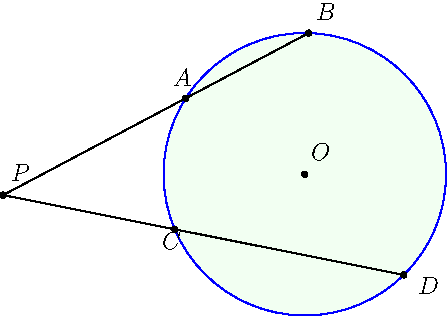
\includegraphics{pop-case1.pdf}
	\qquad
		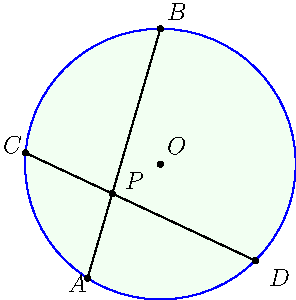
\includegraphics{pop-case2.pdf}
	\caption{Power of a Point}
\end{figure}


\section{Radical Axis}
What is radical axis? Radical axis is a set of points which have equal power with respect to two circles. It is a straight line and easy to prove using cartesian co-ordinates.

It is easy to draw the radical axis of two intersecting circles, but if thye are not intersecting then we have to draw another circelwhich intersect the two circles, then by the radical center, we can find hte radical axis.


Suppose that we have given three distinct circle, where pairwise radical axes are not parallel then they must concur. This (the point of concurrency) is called \vocab{Radical Center} of three circles.


Now we are going to see some example of problem solving using power of a point.

\begin{example}
Let $ABC$ be an acute triangle. Let the line through $B$ perpendicular to $AC$ meet the
circle with diameter $AC$ at points $P$ and $Q$, and let the line through $C$ perpendicular
to $AB$ meet the circle with diameter $AB$ at points $R$ and $S$. Prove that $P, Q, R, S$ are
concyclic.
\end{example}

\begin{figure}[ht]
\centering
	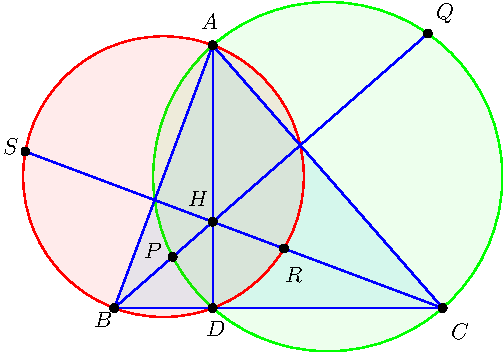
\includegraphics{radax-prob2.pdf}%[scale=0.5]{pop-prob1.png}
	\caption{Soving a problem using PoP}
\end{figure}


\begin{soln}
Let $D$ be the foot of the perpendicular from $A$ to $BC$ andlet $H$ be the orthocenter of $ABC$. Since, $\angle ADB =90\dg$, the circle with diameter $AB$ passes through $D$, so $HS \cdot HR =
HA \cdot HD$ by power of a point. 

Similarly the circle with diameter $AC$ passes through $D$
as well, so $HP \cdot HQ = HA \cdot HD$ as well. Hence $HP \cdot HQ = HR \cdot HS$, and therefore by
the converse of power of a point, $P, Q, R, S$ are concyclic.
\end{soln}

\section{PoP for showing Concurrency}

\begin{example}[IMO 1995]
Let $A, B, C$, and $D$ be four distinct points on a line, in that order. The
circles with diameters $AC$ and $BD$ intersect at $X$ and $Y$ . The line $XY$ meets $BC$ at $Z$.
Let $P$ be a point on the line $XY$ other than $Z$. The line $CP$ intersects the circle with
diameter $AC$ at $C$ and $M$ , and the line $BP$ intersects the circle with diameter $BD$ at $B$
and $N$ . Prove that the lines $AM , DN$ , and $XY$ are concurrent.
\end{example}

\begin{figure}[ht]
\centering
	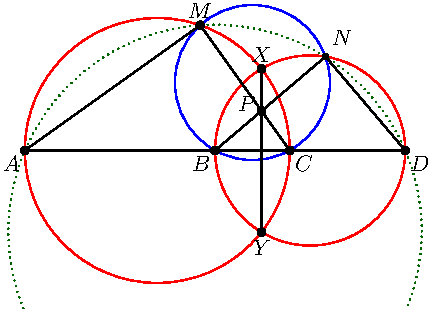
\includegraphics{pop-concur.pdf}%[scale=0.5]{pop-concur.png}
	\caption{PoP for showing Concurrency}
\end{figure}

\begin{soln}
By power of a point we have \(PM \cdot PC= PX\cdot PY =PN \cdot PB \). So, \(B,C,M,N\) are concyclic. Note that $\angle AMC = \angle BND = 90\dg$ since they are subtended by diameters $AC$ and $BD$, respectively. Hence $\angle MND = 90\dg + \angle MNb = 90\dg + \angle MCA = 180\dg -\angle MAD $.

Therefore, $A,D,N,M$ are concyclic. Since $AM,DN,XY$ are thethree radical axes for the circumcircles of $AMXC,BXND$ and $AMND$, they concur at the radical center.

\end{soln}

\section{PoP for showing Collinearity}

\begin{example}
Let $ABC$ be a triangle and let $D$ and $E$ be points on the sides $AB$ and $AC$, respectively,
such that $DE$ is parallel to $BC$. Let $P$ be any point interior to triangle $ADE$, and let $F$
and $G$ be the intersections of $DE$ with the lines $BP$ and $CP$ , respectively. Let $Q$ be the
second intersection point of the circumcircles of triangles $PDG$ and $PFE$. Prove that the
points $A, P$, and $Q$ are collinear.
\end{example}

\begin{figure}[ht]
\centering
	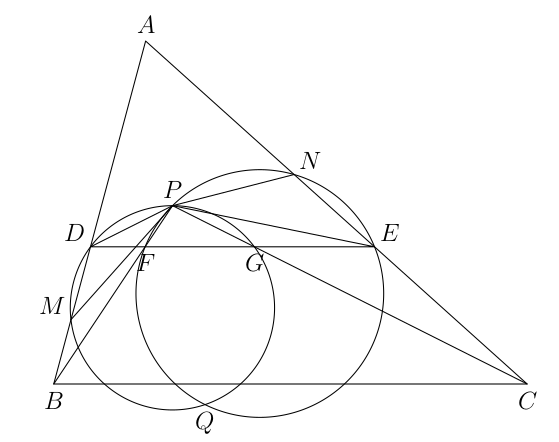
\includegraphics[scale=0.3]{pop-collinear.png}
	\caption{PoP for showing Collinearity}
\end{figure}

\begin{soln}
Let the circumcircle of $DPG$ meet line $AB$ again at $M$ , and let the circumcircle of $EPF$
meet line $AC$ again at $N$ . Assume the configuration where $M$ and $N$ lie on sides $AB$
and $AC$ respectively (the arguments for the other cases are similar). We have $\angle  ABC =
\angle  ADG = 180 \dg - \angle  BDG = 180 \dg - \angle M P C,$ so $BMPC$ is cyclic. Similarly, $BPNC$ is
cyclic as well. So $BCNPM$ is cyclic. Hence $\angle AN M = \angle ABC = \angle ADE,$ so $M, N, D, E$
are concyclic. By power of a point, $AD \cdot AM = AE \cdot AD$. Therefore, $A$ has equal power
with respect to the circumcircles of $DPG$ and the $EPF$ , and thus $A$ lies on line $PQ$, the radical axis.

\end{soln}

Here I am going to include some problems which can be solved using Power of a Point.
\begin{problem}[IMO 2000/1]
Two circles $G_1$ and $G_2$ intersect at two points $M$ and $N$ . Let
$AB$ be the line tangent to these circles at $A$ and $B$, respectively, so that $M$ lies closer to $AB$
than $N$ . Let $CD$ be the line parallel to $AB$ and passing through the point $M$, with $C$ on $G_1$
and $D$ on $_2$ . Lines $AC$ and $BD$ meet at $E$; lines $AN$ and $CD$ meet at $P$ ; lines $BN$ and
$CD$ meet at $Q$. Show that $EP = EQ$.
	\begin{hint}
		\addhint{}
		\addhint{}	
	\end{hint}
\end{problem}

\begin{problem}[USAMO 1997/2]
Let $ABC$ be a triangle. Take points $D, E, F$ on the
perpendicular bisectors of $BC, CA, AB$ respectively. Show that the lines through $A, B, C$
perpendicular to $EF , F D, DE$ respectively are concurrent.
	\begin{hint}
		\addhint{}
		\addhint{}	
	\end{hint}
\end{problem}

\begin{problem}[USAJMO 2012/1]
Given a triangle $ABC$, let $P$ and $Q$ be points on segments
$AB$ and $AC$, respectively, such that $AP = AQ$. Let $S$ and $R$ be distinct points on segment
$BC$ such that $S$ lies between $B$ and $R$, $\angle BPS = \angle PRS$, and $\angle CQR = \angle QSR$. Prove
that $P , Q, R, S$ are concyclic.
	\begin{hint}
		\addhint{}
		\addhint{}	
	\end{hint}
\end{problem}
%\section{}

%\section{}

%\section{}
